\documentclass{fkssolpub}

\usepackage[czech]{babel}
\usepackage{fontspec}
\usepackage{fkssugar}
\usepackage{amsmath}
\usepackage{graphicx}

\author{Ondřej Sedláček}
\school{Gymnázium Oty Pavla} 
\series{2}
\problem{A} 

\begin{document}

\begin{figure}
	\begin{center}
		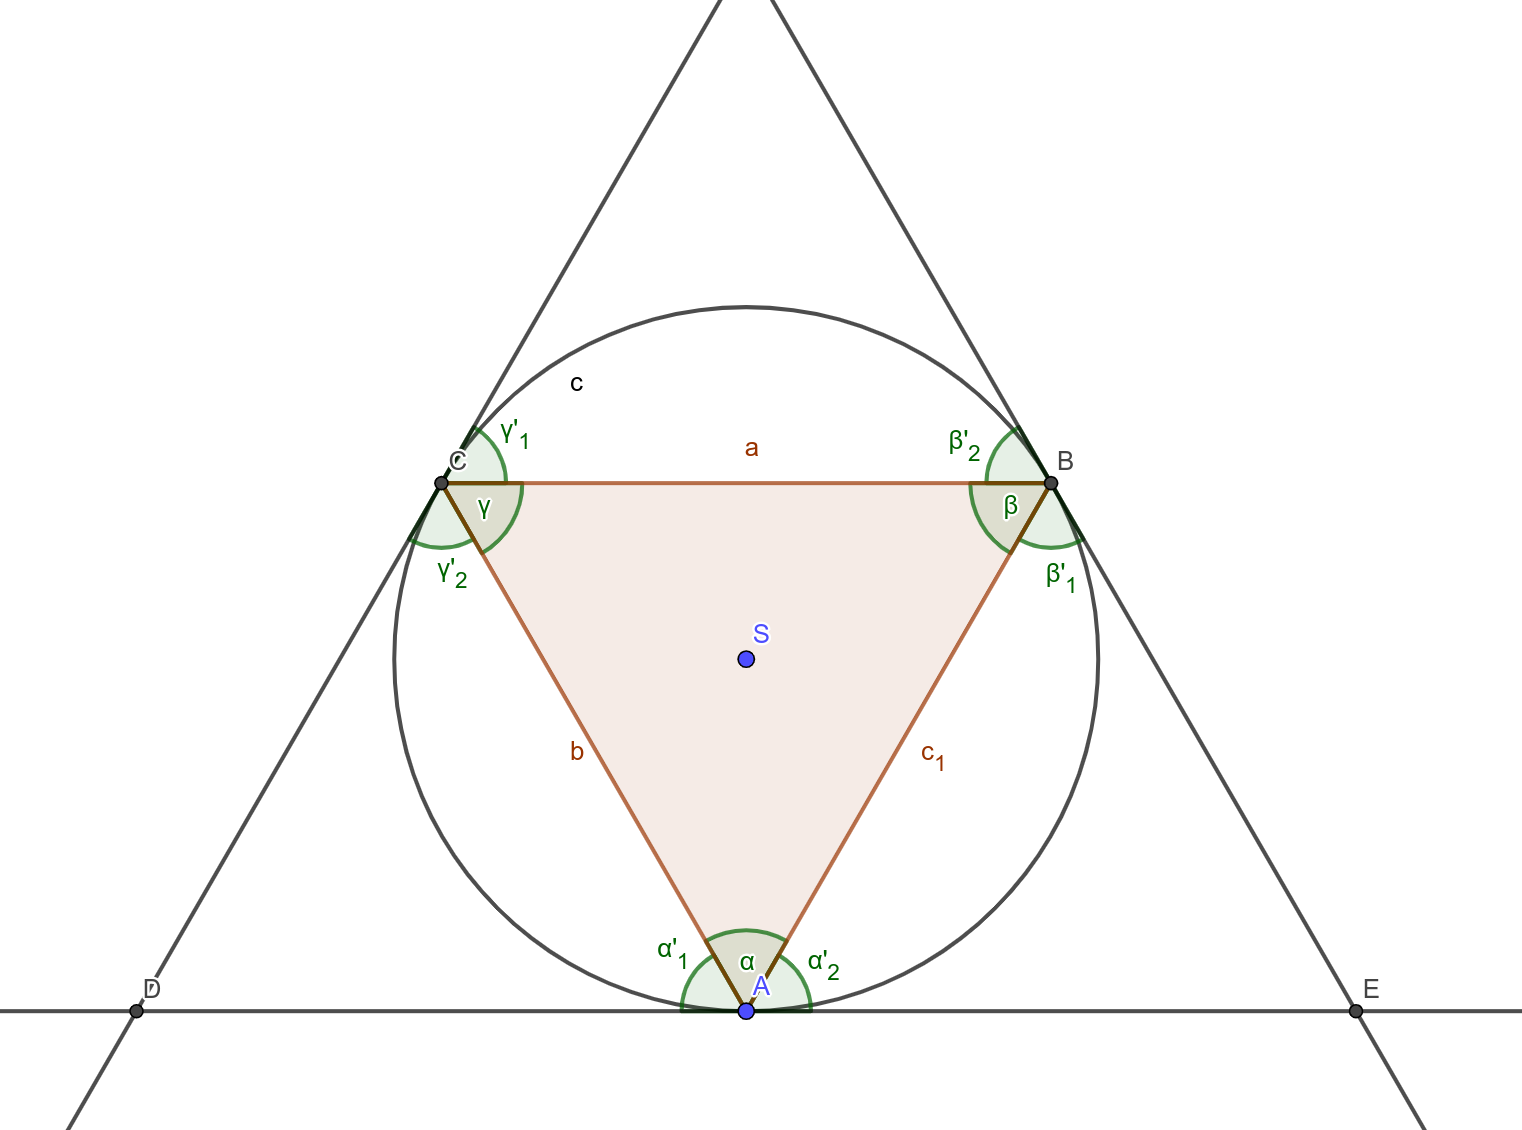
\includegraphics[width=0.95\textwidth]{A-fig}
	\end{center}
	\caption{Konstrukce úlohy}
	\label{fig:1}
\end{figure}

Protože se kulka odráží od kružnice jako světlo, v náčrtku \ref{fig:1} pak platí, že $\alpha'_1 = \alpha'_2$, $\beta'_1 = \beta'_2$, $\gamma'_1 = \gamma'_2$. Zároveň z věty o úsekovém úhlu víme, že $\alpha'_2 = \beta'_1$, $\beta'_2 = \gamma'_1$, $\gamma'_2 = \alpha'_1$. Z toho ale víme, že všechny tyto úhly jsou si rovny, a tedy:

\[
	\alpha'_1 = \alpha'_2 = \beta'_1 = \beta'_2 = \gamma'_1 = \gamma'_2
\]

Z toho pak zřejmě platí, že:

\[
	180^{\circ} - \alpha'_1 - \alpha'_2 = \alpha = \beta = \gamma
\]

Aby pak platilo, že $\alpha + \beta + \gamma = 180^{\circ}$, musí tedy $\alpha = \beta = \gamma = 60 ^{\circ}$ a proto i zbývající úhly musí být $60^{\circ}$. Tedy abychom splnili zadání, musíme vystřelit pod úhlem $60 ^{\circ}$ a $120^{\circ}$.


\end{document}
